\subsection{¿Se pueden construir modelos útiles?}
\subsubsection*{Objetivos, variables y muestras comunes}
Se evalúa (i) estimar lluvia mensual local de Zaragoza-AUT a partir de IMERG o CHIRPS y (ii) estimar el caudal medio mensual Q a partir de cada producto de precipitación; se añade la relación local--Q como ejercicio exploratorio. P(t) es precipitación de cuenca en mm/mes, L(t) lluvia local en mm/mes y Q(t) caudal en m$^3$/s. IMERG es el promedio del polígono exacto. Las dos fuentes usan las mismas fechas para cada comparación. Para modelos con rezago se exige Q, P\_IMERG(t), P\_CHIRPS(t) y ambas lluvias en t-1 válidas: quedan 274 meses de 1998--2022, once menos que los 285 pares contemporáneos de 2.1. No se rellenan faltantes. Hay 206 meses para desarrollo hasta diciembre de 2016 y 68 meses de 2017--2022 reservados para el 2.3, sin evaluar sus resultados.
\subsubsection*{Relaciones candidatas y criterio de selección}
La nube positiva de 2.1 justifica probar una recta como referencia, sin suponer que determine una respuesta única. Se comparan media constante, climatología mensual, Q=a+bP(t), Q=a+bP(t-1), Q=a+bP(t)+cP(t-1) y Q=a+b$\sqrt{\vphantom{P}}$P(t). La raíz cuadrada es una alternativa no lineal sencilla para una posible respuesta sublineal y no transforma el caudal. Se ajusta por mínimos cuadrados con intercepto, sin forzar paso por el origen. La selección usa RMSE agregado de tres validaciones temporales dentro del desarrollo: ajuste hasta 2006$\rightarrow$2007--2009, hasta 2009$\rightarrow$2010--2012 y hasta 2012$\rightarrow$2013--2016 (29, 30 y 46 meses, total 105). Cada coeficiente, media y climatología se estima solo con el pasado de su bloque. Se prefieren dos parámetros si el tercero mejora menos del 5 \%; se considera candidato útil si reduce al menos 5 \% el RMSE frente al mejor referente sin lluvia. Este umbral es una regla práctica explícita, no una prueba de significancia. La evaluación final independiente de 2017--2022 se realizará en 2.3.
\begin{center}\small\begin{tabular}{rrrrrrr}\hline
Fuente & Modelo & n & RMSE & MAE & Sesgo & $R^2$ \\ \hline
IMERG & Media constante & 105 & 83,17 & 60,06 & -2,25 & -0,04 \\
IMERG & Climatología mensual & 105 & 77,37 & 56,24 & -4,92 & 0,10 \\
IMERG & Lineal P(t) & 105 & 63,45 & 43,08 & -16,02 & 0,39 \\
IMERG & Lineal P(t-1) & 105 & 67,38 & 42,75 & -15,84 & 0,32 \\
IMERG & P(t) + P(t-1) & 105 & 56,43 & 38,97 & -22,66 & 0,52 \\
IMERG & Raíz de P(t) & 105 & 65,14 & 44,82 & -17,16 & 0,36 \\
CHIRPS & Media constante & 105 & 83,17 & 60,06 & -2,25 & -0,04 \\
CHIRPS & Climatología mensual & 105 & 77,37 & 56,24 & -4,92 & 0,10 \\
CHIRPS & Lineal P(t) & 105 & 69,42 & 48,58 & -2,19 & 0,27 \\
CHIRPS & Lineal P(t-1) & 105 & 71,36 & 50,57 & -3,21 & 0,23 \\
CHIRPS & P(t) + P(t-1) & 105 & 63,87 & 45,99 & -2,81 & 0,38 \\
CHIRPS & Raíz de P(t) & 105 & 70,19 & 49,80 & -3,91 & 0,26 \\
\hline\end{tabular}\end{center}
\subsubsection*{Resultado para caudal: modelos con lluvia actual y antecedente}
El modelo con P(t) y P(t-1) es el candidato seleccionado para ambas fuentes: mejora la recta contemporánea y los referentes de media y climatología. IMERG obtiene RMSE 56,43 m$^3$/s, MAE 38,97 y R$^2$ 0,52 en los 105 meses de validación de desarrollo; CHIRPS obtiene RMSE 63,87, MAE 45,99 y R$^2$ 0,38. La climatología tiene RMSE 77,37; la reducción es 27,1 \% para IMERG y 17,4 \% para CHIRPS. La raíz de P no supera al modelo con rezago. Esta evidencia respalda utilidad preliminar, no certifica predicción operativa. Las ecuaciones siguientes corresponden al reajuste final con los 206 meses de desarrollo; las métricas anteriores proceden de coeficientes ajustados por separado en cada bloque.
\[\widehat{Q}_t=\max\left(0,-87.2692+0.465439P_{IMERG,t}+0.433065P_{IMERG,t-1}\right).\]
\[\widehat{Q}_t=\max\left(0,-35.8526+0.422155P_{CHIRPS,t}+0.434939P_{CHIRPS,t-1}\right).\]
\begin{figure}[H]\centering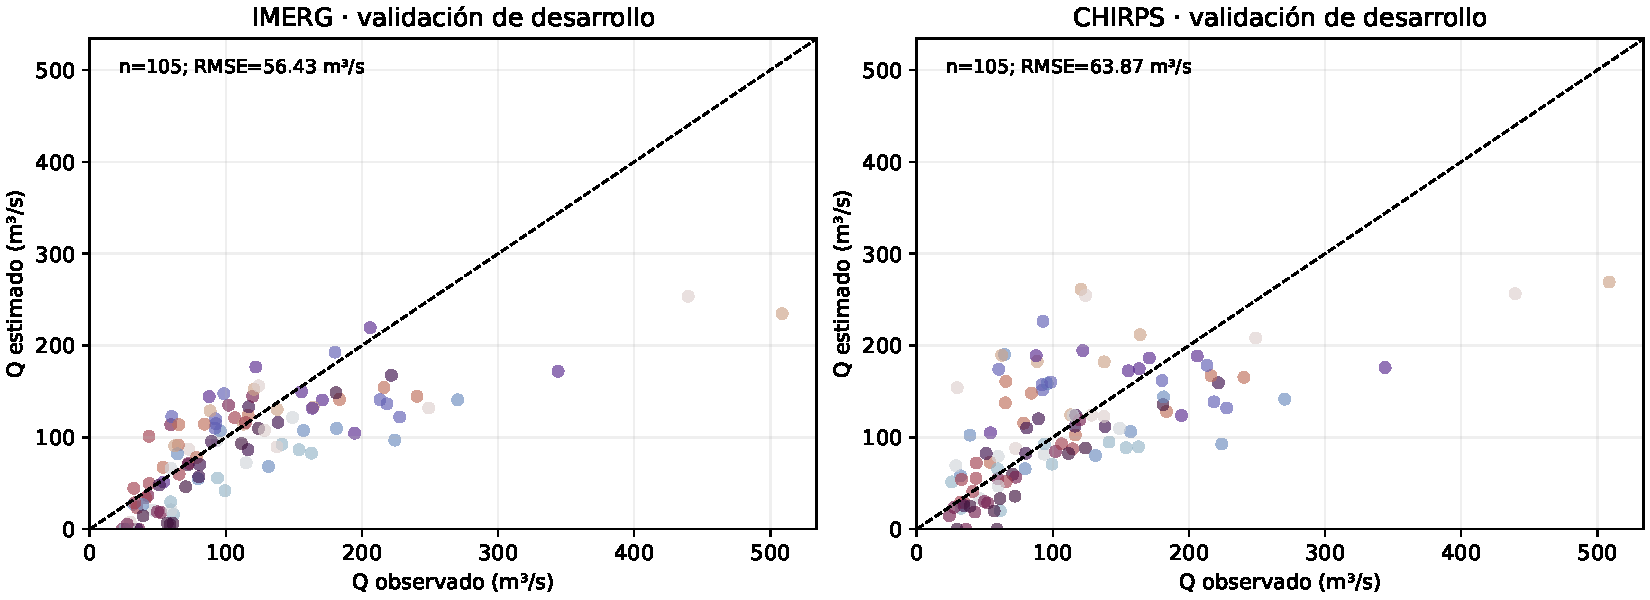
\includegraphics[width=\linewidth]{../apartado_2_2/modelos_Q_comparados.pdf}\caption{Modelos de caudal: validación temporal dentro del desarrollo.}\end{figure}
\begin{figure}[H]\centering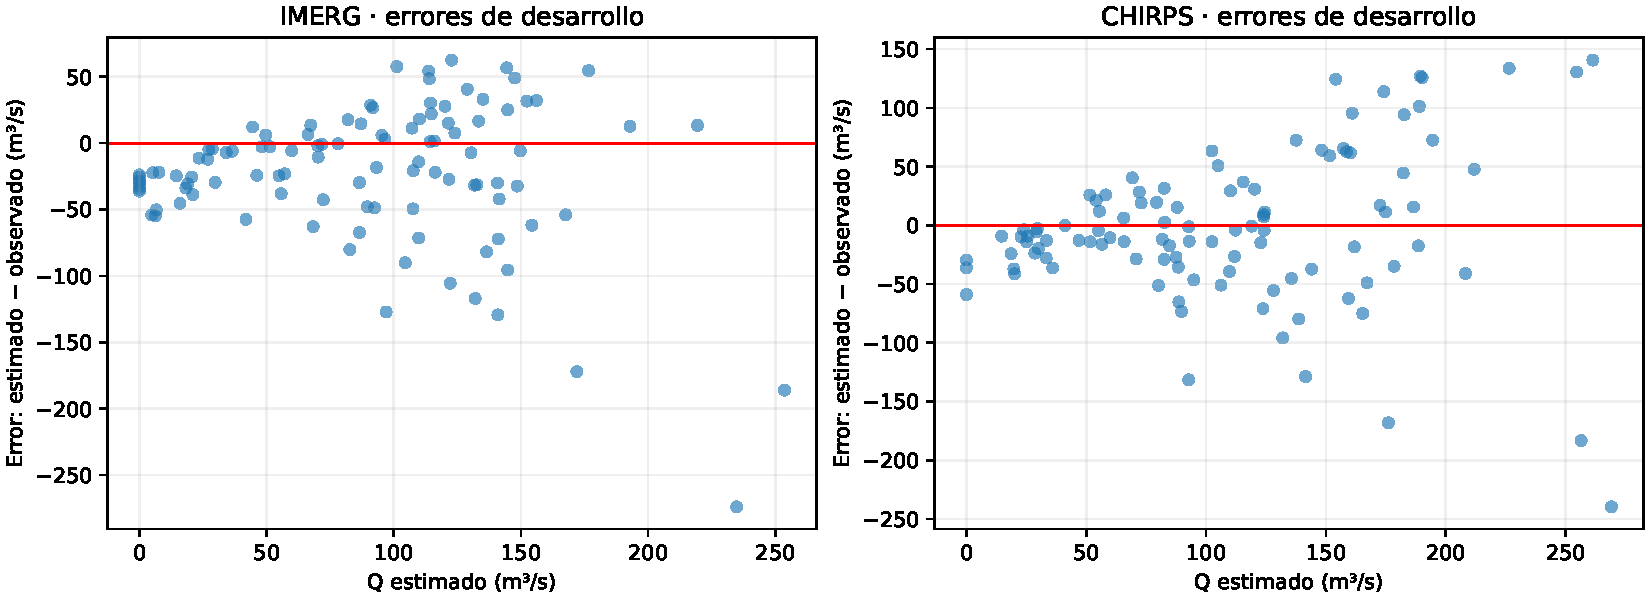
\includegraphics[width=\linewidth]{../apartado_2_2/residuos_Q.pdf}\caption{Errores de estimación de caudal durante la validación de desarrollo.}\end{figure}
\begin{center}\small\begin{tabular}{rrrrr}\hline
Fuente & Modelo & a & b & c \\ \hline
IMERG & Lineal P(t) & -26,10 & 0,61 & 0,00 \\
IMERG & Lineal P(t-1) & -22,11 & 0,60 & 0,00 \\
IMERG & P(t) + P(t-1) & -87,27 & 0,47 & 0,43 \\
IMERG & Raíz de P(t) & -138,95 & 16,97 & 0,00 \\
CHIRPS & Lineal P(t) & 10,97 & 0,57 & 0,00 \\
CHIRPS & Lineal P(t-1) & 9,20 & 0,59 & 0,00 \\
CHIRPS & P(t) + P(t-1) & -35,85 & 0,42 & 0,43 \\
CHIRPS & Raíz de P(t) & -70,49 & 14,11 & 0,00 \\
\hline\end{tabular}\end{center}
\subsubsection*{Lluvia local: calibración sencilla y evidencia limitada}
Se conserva solo la cobertura 100 \%: 14 meses completos. Para cada producto se comparan media, recta y raíz de P. La recta es la referencia elegida por parsimonia: la raíz no muestra una mejora convincente con tan pocos datos. En ajuste sobre los 14 meses, RMSE es 35,87 mm/mes para IMERG y 33,59 para CHIRPS. En un diagnóstico temporal muy corto (siete meses de 2018 para ajustar y siete de 2019 para comprobar), las rectas dan RMSE 41,85 para IMERG y 30,50 para CHIRPS; el referente constante da 58,03. Para IMERG, la raíz apenas mejora ese diagnóstico un 0,9 \%, insuficiente para preferirla; para CHIRPS empeora. No se selecciona por correlación ni se presenta el ajuste como validación. Estas ecuaciones calibran un promedio de cuenca hacia una estación puntual; no reconstruyen automáticamente la lluvia verdadera de toda la cuenca ni autorizan extrapolar a otras estaciones. Las ecuaciones mostradas usan los 14 meses, mientras la comprobación temporal usó únicamente coeficientes de 2018.
\[\widehat{L}_t=\max\left(0,-30.7549+0.596818P_{IMERG,t}\right).\]
\[\widehat{L}_t=\max\left(0,-0.9713+0.504221P_{CHIRPS,t}\right).\]
\begin{center}\small\begin{tabular}{rrrrrr}\hline
Fuente & Modelo & RMSE ajuste & RMSE temporal & MAE temporal & $R^2$ temporal \\ \hline
IMERG & Media constante & 58,28 & 58,03 & 48,58 & -0,04 \\
IMERG & Lineal P(t) & 35,87 & 41,85 & 36,76 & 0,46 \\
IMERG & Raíz de P(t) & 36,25 & 41,47 & 36,76 & 0,47 \\
CHIRPS & Media constante & 58,28 & 58,03 & 48,58 & -0,04 \\
CHIRPS & Lineal P(t) & 33,59 & 30,50 & 25,58 & 0,71 \\
CHIRPS & Raíz de P(t) & 34,26 & 33,09 & 30,23 & 0,66 \\
\hline\end{tabular}\end{center}
\begin{figure}[H]\centering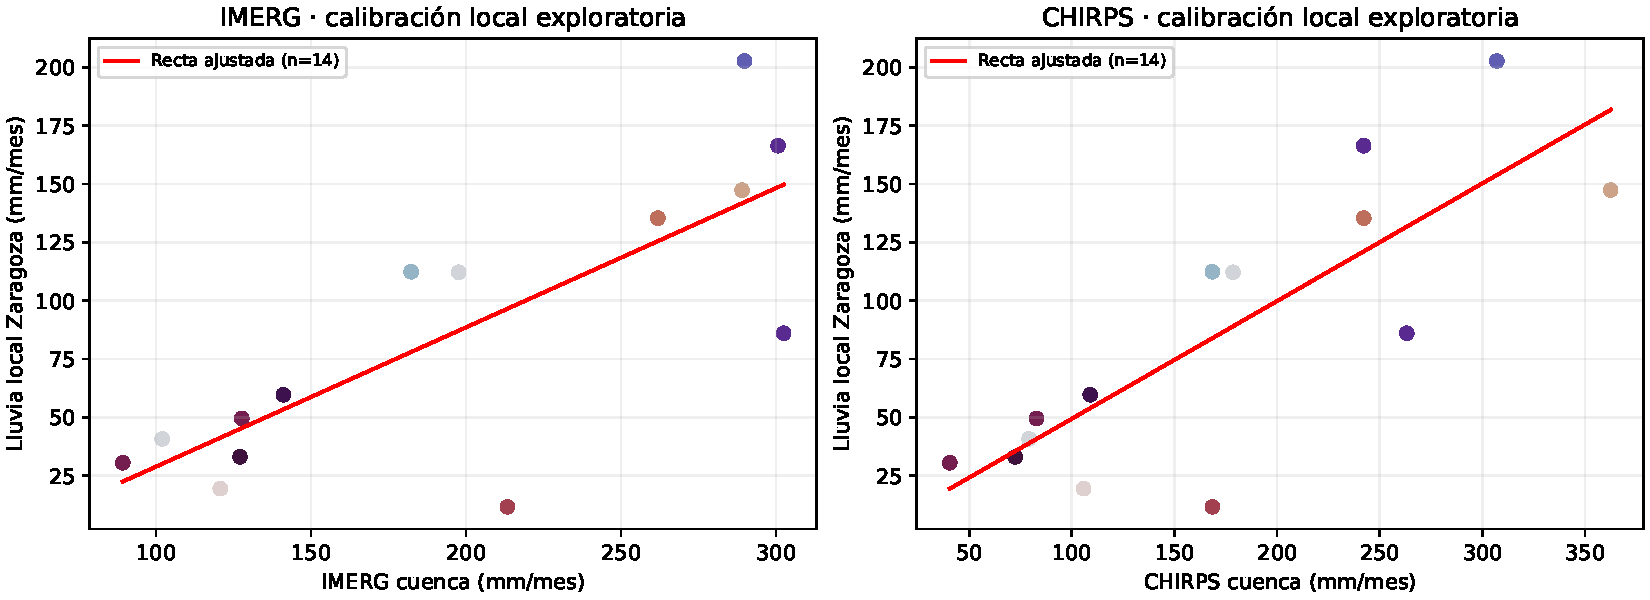
\includegraphics[width=\linewidth]{../apartado_2_2/modelos_lluvia_local.pdf}\caption{Calibraciones locales exploratorias, catorce meses de ajuste.}\end{figure}
\subsubsection*{Caudal a partir de lluvia local: no recomendar todavía}
La recta local--Q con 14 pares da RMSE de ajuste 51,13 m$^3$/s. En el diagnóstico temporal de siete meses de 2019, RMSE es 54,31 y R$^2$ solo 0,03, con sesgo +39,05 m$^3$/s; el referente constante tiene RMSE 71,01. La raíz empeora a RMSE 57,88 y R$^2$ negativo. Aunque la recta reduce error respecto de esa media, la explicación de la variabilidad es escasa, el sesgo es grande y el registro demasiado corto. Se documenta la ecuación exploratoria, pero no se recomienda un modelo operativo local--Q ni añadirle más parámetros o rezagos con esta muestra. No se compara directamente su RMSE de siete meses con los RMSE de 105 meses de IMERG/CHIRPS.
\[\widehat{Q}_t=\max\left(0,55.3322+0.654768L_t\right).\]
\begin{center}\small\begin{tabular}{rrrrr}\hline
Modelo & RMSE ajuste & RMSE temporal & Sesgo temporal & $R^2$ temporal \\ \hline
media & 63,80 & 71,01 & 44,69 & -0,66 \\
lineal & 51,13 & 54,31 & 39,05 & 0,03 \\
raiz & 52,81 & 57,88 & 41,74 & -0,10 \\
\hline\end{tabular}\end{center}
\subsubsection*{Supuestos, rangos, ceros y transformaciones}
El modelo supone una relación aproximadamente estable en el periodo y ámbito de calibración; cambios de medición, uso del suelo, extracciones, humedad antecedente y regulación pueden romperla. Mínimos cuadrados minimiza errores cuadrados y es sensible a extremos. No se supone independencia de meses para calcular p-valores ni intervalos; los residuos pueden ser autocorrelacionados y de varianza cambiante. P(t-1) significa estrictamente el mes anterior del calendario, sin saltar faltantes. Las precipitaciones y caudales cero, si estuvieran observados, serían válidos; en las muestras actuales no hay ceros. La raíz admite cero y evita añadir constantes arbitrarias. Los faltantes nunca se sustituyen por cero. Para evitar estimaciones físicas negativas se publica max(0, expresión), también aplicado durante la comparación; no se recorta el extremo superior. No se recomienda extrapolar fuera de los rangos observados. Las ecuaciones con P(t) estiman el caudal una vez conocida la lluvia del mismo mes: no son pronósticos adelantados.
\begin{center}\small\begin{tabular}{rrrrr}\hline
Fuente & P mín. Q & P máx. Q & P mín. local & P máx. local \\ \hline
IMERG & 60,83 & 440,52 & 89,28 & 302,46 \\
CHIRPS & 30,12 & 396,03 & 40,56 & 362,47 \\
\hline\end{tabular}\end{center}
Rango de Q en desarrollo: 21,34--508,77 m$^3$/s.
\subsubsection*{Interpretación de parámetros y conservación de masa}
En lluvia local, el intercepto tiene unidades mm/mes y la pendiente es adimensional. En caudal, el intercepto está en m$^3$/s y las pendientes en (m$^3$/s)/(mm/mes); el coeficiente de $\sqrt{\vphantom{P}}$P tendría unidades (m$^3$/s)/$\sqrt{\vphantom{P}}$(mm/mes). Una pendiente positiva indica asociación, no una fracción causal de lluvia convertida en caudal. El intercepto negativo y el truncamiento no representan un balance de agua. Q estimado puede convertirse a lámina mensual con R\_est=86,4$\times$días\_del\_mes$\times$Q\_est/2797,19, pero la regresión no conserva masa: faltan evapotranspiración, cambios de almacenamiento, aportes, extracciones y controles de operación. No se interpreta P(t-1) como un tiempo de viaje medido.
\subsubsection*{Comparación y decisión del apartado 2.2}
Para lluvia local, la recta CHIRPS tiene mejor desempeño en el diagnóstico disponible, pero la muestra de 14 meses exige tratarla como calibración exploratoria. Para caudal, IMERG con lluvia actual y antecedente tiene menor RMSE y MAE de desarrollo que CHIRPS. Sin embargo, su sesgo es -22,66 m$^3$/s, frente a -2,81 de CHIRPS: menor error cuadrático no implica menor sesgo. Los gráficos de residuos permiten revisar magnitud y persistencia del error; no se prometen intervalos de predicción sin validación. Se proponen dos candidatos de caudal para pasar al 2.3, se mantienen calibraciones locales exploratorias y se descarta afirmar que la lluvia local corta sustenta un modelo operativo. Los 68 meses reservados quedan intactos para comprobar generalización, extremos y estabilidad.
\begin{center}\small\begin{tabular}{rrrr}\hline
Fuente & r error antecedente & RMSE Q alto & Sesgo Q alto \\ \hline
IMERG & 0,53 & 98,29 & -76,29 \\
CHIRPS & 0,67 & 89,13 & -63,59 \\
\hline\end{tabular}\end{center}
